\chapter{Hardware-Aware Analysis}\label{quantization}
In this chapter, the hardware-aware optimizations used in the FPGA implementations are first presented and then their application in the proposed architectures is explained. Other elements of the hardware design and configuration process are then described which results in a comprehensive picture of the FPGA-mapped architectures. Afterwards, two analytical models are considered - one for the latency and the other for the resource utilization. The custom post-training quantization tool is discussed along with its suitability for this project. Then, existing infrastructure that ties together higher and lower-level code representation is introduced along with its synergy with a High-Level Synthesis optimization tool chain. Lastly, the technical contributions to \hlsml library are listed and explained.

\section{Hardware-Aware Optimizations}

\subsection{Tensor Multiplication and Scaling}\label{tensor-multiplication}
Each self-attention head performs two tensor multiplications (referred to as \textit{matmul} blocks in figure \ref{fig:self-attention-multi-head}), which are normally expressed using Einstein Summation notation \cite{59-barr1991einstein}, which is supported by mathematical and machine learning libraries like \texttt{NumPy} or \texttt{PyTorch}. However, not present by default in HLS, it requires careful design of the calculation loops in order to not cripple the performance by unnecessary computations and pseudo-random data accesses. As part of this research, an efficient and fully-customizable HLS block has been designed, that uses a very similar interface to the Python equivalent.

\begin{figure}[hpt!]
  \centering
  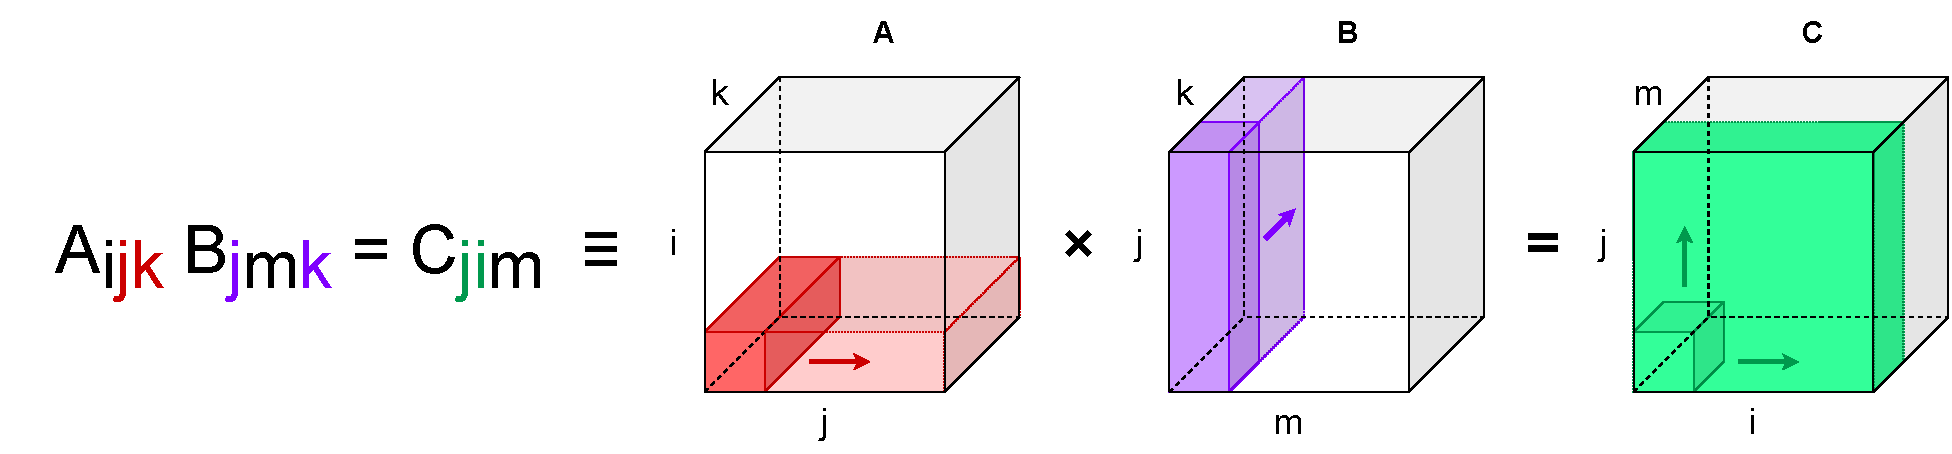
\includegraphics[trim={0cm 0cm 0cm 0cm}, width=0.75\textwidth, center]{models/einsum.pdf}
  \caption{Visualization of a tensor operation expressed in Einstein Summation notation.}
  \label{fig:einsum}
\end{figure}

Figure \ref{fig:einsum} shows a visualization for an example notation to give a better understanding of the necessary flexibility of a formula. The translation between notations using the custom tool is showcased in listing \ref{list:einsum}. While the \texttt{PyTorch} implementation can often use 4-dimensional tensors, the first dimension refers to the batch, which is not present in the hardware implementation that processes input samples one-by-one, hence both the figure and code listing show 3-dimensional cases. It is also worth pointing out, that tensor multiplication is an inherently computationally expensive operation due to the quadruple-nested loop structure. For this reason, the proposed design leaves the configuration of pipelining as a parameter that offers a trade-off between time and design complexity. The \textit{design} complexity refers to the difficulty involved in HLS synthesis as well as hardware resource utilization. In other words, the hardware block can be instantiated to run serially, where little resources are needed as they get re-used, or alternatively, in parallel, where significantly more components are used to decrease latency, and in case the design is also pipelined, to also increase throughput.

% \clearpage
\lstinputlisting[language={[GNU]C++}, caption={From PyTorch \texttt{out = torch.einsum("qhc,khc->hqk", [A, B])} to HLS C++ code.}, captionpos=b, label={list:einsum}]{quantization/einsum_example.cpp}

\begin{equation}\label{eq:einsum-no-unrolling}
  \text{Design}: \mathcal{O}(n) \quad \text{Time}: \mathcal{O}(HKQC \cdot n)
\end{equation}

Let's consider the two extreme cases for the design - no loop unrolling and complete unrolling, where the latter is required for the block to be fully pipelined, and assume that multiply-accumulate and addition both have \(n\) time and space complexity. In the first case, a single multiply-accumulate operation happens at once, hence a final result is only available after all the loops have been fully iterated, with complexities shown in \ref{eq:einsum-no-unrolling}.

\begin{equation}\label{eq:einsum-full-unrolling}
  \text{Design}: \mathcal{O}(HKQC \cdot n) \quad \text{Time}: \mathcal{O}(n \cdot \log (HKQC))
\end{equation}

In the second one, all loop operations can execute at the same time, although the intermediate results need to be summed accordingly using an adder tree (seen in figure \ref{fig:adder-tree}) which has a logarithmic time and linear space complexity, before saving the output tensor, which leads to complexities seen in \ref{eq:einsum-full-unrolling}. The time complexity may appear high, but it has to be remembered that unrolling allows for the pipelining of this design, which cannot decrease latency, but can vastly increase throughput, as each addition can happen in a single cycle.

\begin{figure}[hpt!]
  \centering
  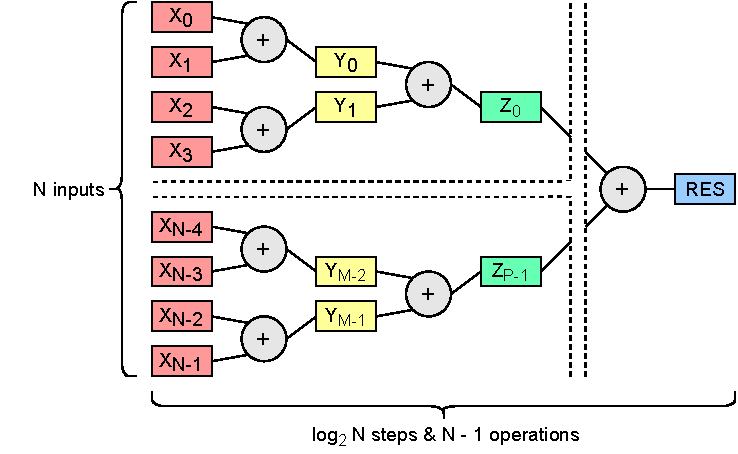
\includegraphics[trim={0cm 0cm 0cm 0cm}, width=0.51\textwidth, center]{quantization/adder_tree.pdf}
  \caption{Illustration of an adder tree with \(N\) inputs.}
  \label{fig:adder-tree}
\end{figure}

Another simple optimization used alongside the tensor multiplication blocks was the change in size scaling from using division to performing an arithmetic right shift (ASR), which requires precomputing the logarithm of the size, seen in equation \ref{eq:log-div}, vastly simplifying the otherwise computationally expensive hardware required at run-time.

\begin{equation}\label{eq:log-div}
  \frac{x}{\sqrt{\text{size}}} \equiv \text{ASR}(x,\; \log_2 \sqrt{\text{size}}) \equiv \text{ASR}(x,\; \frac{1}{2}\log_2 \text{size})
\end{equation}


\subsection{Softmax and Log Softmax Activations}\label{log-softmax}
Despite an already existing \hlsml implementation of the softmax activation function, computing the logarithm of its result is not as simple as it may seem. This is because the numerical stability and computational efficiency of this operation is often explored in-depth \cite{60-blanchard2019accurate} and varies depending on the programming language and target platform.

\begin{figure}[hpt!]
  \centering
  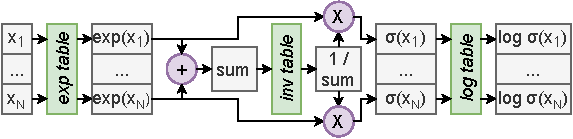
\includegraphics[trim={0cm 0cm 0cm 0cm}, width=0.55\textwidth, center]{quantization/log_softmax_naive_h.pdf}
  \caption{Direct hardware implementations of log softmax.}
  \label{fig:log-softmax-naive}
\end{figure}

The naive implementation comes straight from the definition of taking a logarithm of softmax, seen in equation \ref{eq:softmax}, and the required hardware operations are shown in figure \ref{fig:log-softmax-naive}.

\begin{equation} \label{eq:softmax}
    \sigma (x_i) = e^{x_i} / \sum_{j=1}^{N} e^{x_j}
\end{equation}

This report proposes a different way of mapping this operation to hardware to improve stability while shortening the critical path and using less resources. It is based on the derivation shown in equation \ref{eq:log-softmax}.

\begin{equation} \label{eq:log-softmax}
    \log (\sigma (x_i)) = log(e^{x_i} / \sum_{j=1}^{N} e^{x_j}) = \log(e^{x_i}) - \log(\sum_{j=1}^{N} e^{x_j}) = e^{x_i} - \log(\sum_{j=1}^{N} e^{x_j})
\end{equation}

The resulting hardware operations are depicted in figure \ref{fig:log-softmax-opt}. It is important to note, that operations like exponentiation, division or taking a logarithm usually rely on precomputing a wide range of values and mapping them in BRAMs or LUTs to allow for lookup on run-time. Hence, the optimized design requires one less of such lookups while also replacing multiplication by a subtraction, which can be simpler to express in hardware.

\begin{figure}[hpt!]
  \centering
  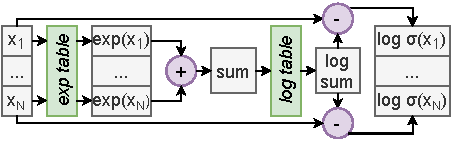
\includegraphics[trim={0cm 0cm 0cm 0cm}, width=0.5\textwidth, center]{quantization/log_softmax_opt_h.pdf}
  \caption{Optimized hardware implementations of log softmax.}
  \label{fig:log-softmax-opt}
\end{figure}

\clearpage
Although further simplifications, including approximating the summation by finding the maximum (see equation \ref{eq:log-softmax-max}) or simply omitting the logarithm portion of the expression, were also explored, they noticeably lowered the final accuracy and were thus abandoned. \todo{Confirm if page breaks correctly.}

\begin{equation} \label{eq:log-softmax-max}
    \log (\sigma (x_i)) = e^{x_i} - \log(\sum_{j=1}^{N} e^{x_j}) = e^{x_i} - \sum_{j=1}^{N} \log(e^{x_j}) = e^{x_i} - \sum_{j=1}^{N} x_j \approx e^{x_i} - \max(x)
\end{equation}


\section{Neural Networks Implementation}
\indo{|}
\indo{|}
\indo{|}

\subsection{Ultra-Low Latency Architecture}
\indo{|}
\indo{|}
\indo{|}
\indo{|}
\indo{|}
\indo{|}

\subsection{Accuracy-Focused Architecture}
\indo{|}
\indo{|}
\indo{|}
\indo{|}
\indo{|}
\indo{|}


\section{Analytical Latency and Resource Models}
In the majority of cases, simulation and synthesis are the best ways of measuring model's accuracy, latency and hardware resources utilization. Although the results might vary compared to an actual FPGA implementation due to various nuances involved in converting the RTL code to equivalent bit stream, the overall design trends remain unchanged. Nonetheless, deriving an analytical model offers a much simpler and easier way of understanding the consequences of modifying a design. While predicting accuracy is not a feasible endeavor due to the complex nature of neural network models, latency estimation is possible for a given design configuration. Tracking hardware resources is not manageable in general as used FF and LUT numbers can reach millions, however, rough estimation of DSP slices can be discussed. In order for the analytical models to be easier to understand and verify, only the smaller, completely pipelined, ultra-low latency architecture is discussed in this section.

\subsection{Latency Model}
A visualization of the architecture annotated with the pipeline stages can be seen in figure \ref{fig:pipeline-stages}. As a consequence of pipelining the model, all the operations can be completed in either one or two cycles. Certain operations like ReLU or scaling share their stage with subsequent components due to their simplicity.

\begin{figure}[hpt!]
  \centering
  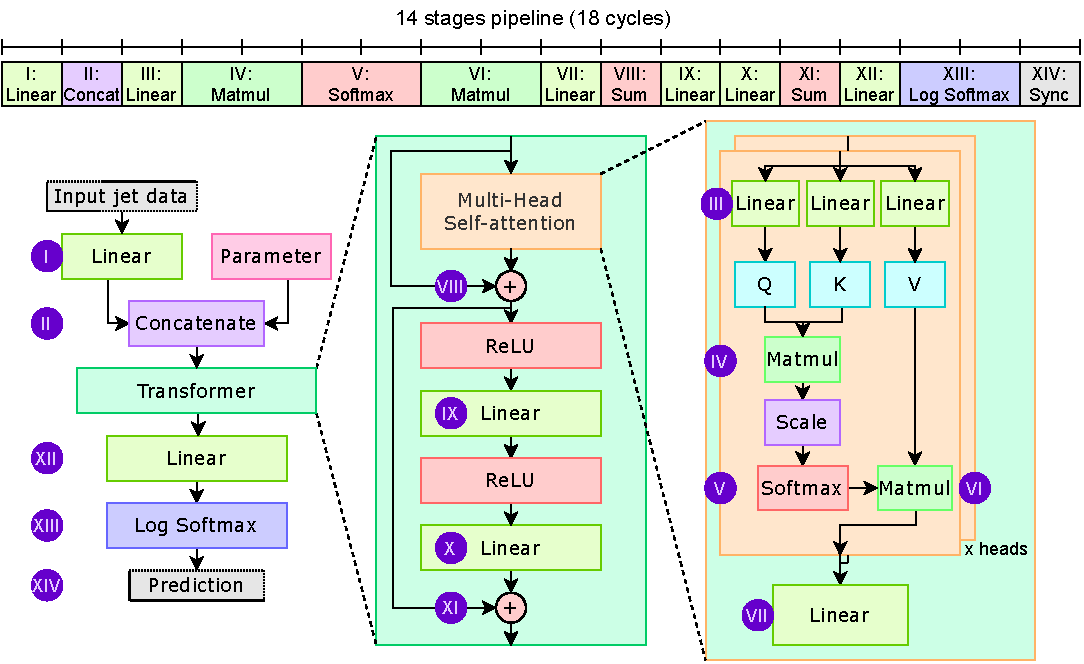
\includegraphics[trim={0cm 0cm 0cm 0cm}, width=1.0\textwidth, center]{quantization/pipelining_stages.pdf}
  \caption{Ultra-low latency architecture with highlighted pipeline stages. Not annotated blocks share stage with their neighbors.}
  \label{fig:pipeline-stages}
\end{figure}

The following components' stages last for two cycles, which suggests that their internal operations could not be completed within a cycle:

\begin{itemize}
  \item Tensor multiplication - a single multiply-accumulate operation requires only one cycle, which might seem counterintuitive at first. However, in this case, several multiplication results need to be added together for each output's value, which leads to additional complexity and latency.
  \item Softmax activation - it performs an exponential function lookup for each input in parallel given the full partitioning of the arrays, but then the values needs to be summed, and more importantly, multiplied, which generates the additional cycle.
  \item Log softmax activation - compared to the previous operation, no multiplication is needed in this case, saving a cycle. However, after the initial lookups, another one needs to happen to find the logarithm value, which requires an additional cycle.
\end{itemize}

The design configuration affects several of the pipeline stages, and hence a significant portion of the latency. The number of transformer layers  have a direct impact on stages III to XI, with each additional layer effectively duplicating them, increasing the latency by \(12\) cycles. Within the transformer block, each feed forward (linear and ReLU) layer contributes one cycle. It is not obvious at first, but the number of self-attention heads do not influence the latency as they are executed in parallel.

\begin{equation} \label{eq:latency-model}
  \text{latency (cycles)} = C_{top} + T \cdot ( C_{SA} + C_{T} + F \cdot C_{FF} )
\end{equation}

Overall, the latency can be expressed using a few variables and constants, leading to the dependency seen in equation \ref{eq:latency-model}. As for the notation, \(C_{top}\), \(C_{SA}\), \(C_{T}\), and \(C_{FF}\) stand for the constant cycles needed in the top-level, self-attention, transformer, and feed-forward components, while \(T\) and \(F\) mean the number of transformers and feed-forward layers.

\begin{equation} \label{eq:latency-model-numbers}
  \text{latency (cycles)} = 6 + 1 \cdot ( 8 + 2 + 2 \cdot 1 ) = 18
\end{equation}

Given the design configuration of the ultra-low latency model, 18 cycles are expected as the overall latency value, as proven in equation \ref{eq:latency-model-numbers}. The number of transformer layers plays the most important role in this model, which can be seen from the plot in figure TODO which shows a 3-dimensional visualization of the latency dependency, with the model's constant values.


\subsection{DSP Model}

% dsp:
% -------
% linear: 240 = 16 x 16 * (15/16) = i x o x coeff
% linear: 75 = 16 x 5 * (15/16) = i x o x coeff
% log softmax: 0 (sub instead of mult)
% trans: 4351
%   relu: 0
%   linear nb: 480 = 16 x 32 * (15/16)
%   linear nb: 705 = 32 x 16 * (1.377 = 705/512)
%   sa: 2162
%     linear qkv: 457 = 32 x 96 * (0.149)
%     matmul: ?
%     scale: 0
%     matmul: ?
%     softmax: 2
%     linear: 244 or 122?


\section{Post-training Quantization}\label{post-training-quantization}
This section returns to the topic of quantization, but as opposed to \cref{pre-training-quantization}, it explores the quantization of already trained models. This is domain is not researched as much as quantization-aware training due to the lack of ability for a model to \textit{compensate} for the quantization noise during training, hence leading to potentially inferior results. However, recent advancements in this field \cite{80-wang2019haq:} leverage the synergy between post-training quantization and the target hardware platform to produce results with improved latency or energy consumption. The inherent noise issues are offset by a careful per-variable bit-width analysis, driven by a reinforcement learning algorithm. The choice of the algorithm has a deep-rooted issue for more computationally demanding models that also require a search in a wider range of bit-widths\footnote{The mentioned method only explores convolutional neural networks in \([1, 8]\) bit-width range.}.

\subsection{Motivation}
This report proposes a novel post-training quantization algorithm that can be applied to state-of-the-art transformer neural networks over a wide precision range. Early tests in the HLS environment revealed that a single C simulation for an input with only 100 samples can take around 10 minutes, which dictates a need for a significantly simpler, hence faster, algorithm than Bayesian optimization or reinforcement learning to allow for an exploration that runs in a reasonable amount of time.

The motivation of the algorithm comes from a hypothesis which states that the neighboring layers in a neural network have a relatively high correlation in their optimal bit-widths. Under this assumption, each layer's input, output, weight, bias and accumulator can be safely explored one-by-one, in the order of appearance in the model. \textit{Safely} refers here to a low likelihood of arriving at a local accuracy extremum that is substantially worse than the global one, that could only theoretically be found using a more sophisticated approach. During this \textit{walk} through the design space, several non-trivial constraints about the widths have to be ensured, which are the topic of the next subsection.

\subsection{Constraints}
The constraints of a network variable could theoretically be set arbitrarily to convey a high-level requirement of an experienced designer with a knowledge about typical widths used for a component in a given network type. However, the proposed method automates this process by extracting the underlying lookup table characteristics to accommodate users without domain-specific expertise. These characteristics are part of the network configuration that ensures that any precomputed (for increased latency) function is stored with adequate precision that avoids introducing unnecessary errors. To give a more concrete example to this abstract definition, one can consider the range of values yielded from the exponential function. Not only is there a set width for the results, but even relatively small values map to numbers that require several bits of integer precision, so careless reduction to either of the width parts can quickly degrade any learning capacity of the model.

\begin{figure}[hpt!]
  \centering
  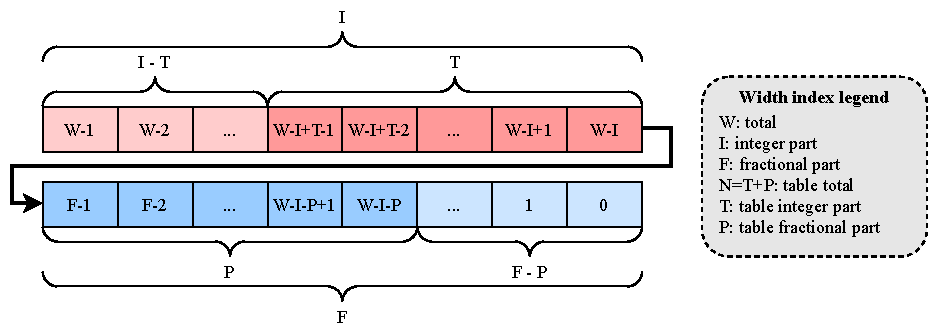
\includegraphics[trim={0cm 0cm 0cm 0cm}, width=1.0\textwidth, center]{quantization/width_constraints.pdf}
  \caption{Visualization of a fixed-point number with its bit-widths as well as constraints imposed by a lookup table. For convenience, red and blue distinguish integer and fractional parts, while the darker hue shows the table-related parts.}
  \label{fig:width-constraints}
\end{figure}

Figure \ref{fig:width-constraints} visualizes a fixed-point number with a detailed analysis of its structure in terms of lookup table constraints, which were added as an optional feature, and are described in \cref{hls4ml-general-purpose}. At first, it could be assumed that the imposed widths should simply be adopted by the variables used by the corresponding table values. However, it is possible for such variables to also have connections to other paths in a network, which can require more precision than the table, hence justifying the existence of the constraints ranges presented in equations \ref{eq:width-constraint-1}, \ref{eq:width-constraint-2}, and \ref{eq:width-constraint-3}, with the notation coming from the corresponding figure.

\begin{equation} \label{eq:width-constraint-1}
  W \geqslant N > T \geqslant 1
\end{equation}
\begin{equation} \label{eq:width-constraint-2}
  W \geqslant I \geqslant T \geqslant 1
\end{equation}
\begin{equation} \label{eq:width-constraint-3}
  W \geqslant F \geqslant P \geqslant 1
\end{equation}

\subsection{Steps}
A high-level overview of the steps used in the proposed method is depicted in algorithm \ref{alg:post-training-quant}. The only required parameters are the negative and positive accuracy tolerance, which are used to guide the search process. Increasing the negative tolerance relaxes the accuracy constraints ensured after each algorithm step in order to significantly reduce the overall bit-widths. On the other hand, a complete opposite objective can also be achieved as reducing the positive tolerance priorities quality of results over narrower bit-widths. Overall, these parameters can take an arbitrary combination of non-negative values that best expresses the exploration goals.

The algorithm starts by scanning an HLS file that includes all the fixed-point types used in a model, convert them into objects and organizes them into a First In, First Out (FIFO) queue, according to their original order. One by one, objects are popped from the queue and undergo the search process. Firstly, the bit-width that was found in the file is saved, the object inherits from the previous optimal bit-width (based on the correlation hypothesis), and the model is evaluated. Depending on whether the results stay within the accuracy tolerance, the object starts with either its original or the inherited configuration. Afterwards, the integer and fractional parts go through one or two loops - first, at each iteration the width gets incremented as long as it matches the target range. After the first loop, the second one, analogous but checking designs with fewer bits, is only entered if no significant improvements were found when increasing widths. This avoids evaluating same configurations unnecessarily, which goes in line with the overall aim to offer a relatively quickly-converging solution to the very multidimensional optimization problem. Once all width objects reach their optimal state, the found configuration is saved and can be used in a further design space exploration.

It is important to point out that the aforementioned PyTorch Eager Mode and FX Graph Mode quantization schemes offer post-training quantization, but there are unsuitable for this work due to their lack of flexibility and support for the essential neural network layers. Instead, the HLS source directory is modified and tested in a C Simulation to measure accuracy. While the synthesis process could supplement the algorithm with an additional feedback signal about the precise hardware resource utilization, it takes much more than the simulation, and its results can be estimated to vary linearly with the total number of bit-widths. The only situation when such assumption does not hold is when a hardware component input width limit is reached because then a 1-bit increase requires an additional instance of that component to be instantiated. Ways of avoiding this issue are covered along with the evaluation of the results in \cref{eval:post-training-quantization}.

\begin{algorithm}
  \caption{Algorithm for performing post-training quantization search}\label{alg:post-training-quant}
  \begin{algorithmic}
  \Function{PostTrainingQuantization}{neg\_accuracy\_tolerance, pos\_accuracy\_tolerance}

  \State $previous\_width \gets null$
  \State $max\_decrement \gets neg\_accuracy\_tolerance \cdot 2$ \Comment{Maximum decrement per parameter}
  \State $optimal\_accuracy \gets$ find\_accuracy()
  \State $params \gets$ scan\_file($defines\_file$) \Comment{FIFO with scanned parameter objects}

  \While{$params$ not empty}
    \State $current \gets params$.pop()

    \If{$previous\_width$ exists} \Comment{Try using width from previous parameter}
      \State $original\_width \gets params.width$
      \State update($params$, $previous\_width$)
      \If{find\_accuracy() $< optimal\_accuracy - max\_decrement$}
        \State update($params$, $original\_width$)
      \Else
        \State $optimal\_accuracy \gets$ find\_accuracy()
      \EndIf
    \EndIf

    \For{$part$ in $\{int, frac\}$}

      \State $try\_increase \gets True$
      \State $pos\_improvement\_found \gets False$
      \While{$try\_increase$} \Comment{Increment to check for high accuracy gain}
        \State $param$.increment($part$)
        \If{find\_accuracy() $ > optimal\_accuracy + pos\_accuracy\_tolerance$}
          \State $optimal\_accuracy \gets$ find\_accuracy()
          \State $pos\_improvement\_found \gets True$
        \Else
          \State $try\_increase \gets False$
          \State $param$.decrement($part$)
        \EndIf
      \EndWhile

      \If{not $pos\_improvement\_found$} \Comment{Decrement if no good increment}
        \State $try\_decrease \gets True$
        \State $acc\_before\_decrease \gets optimal\_accuracy$
        \While{$try\_increase$}
          \State $param$.decrement($part$)
          \If{$acc\_before\_decrease -$ find\_accuracy()$ > max\_decrement$}
            \State $try\_decrease \gets False$
            \State $param$.increment($part$)
          \ElsIf{find\_accuracy() $ > optimal\_accuracy - neg\_accuracy\_tolerance$}
            \State $optimal\_accuracy \gets$ find\_accuracy()
          \Else
            \State $try\_decrease \gets False$
            \State $param$.increment($part$)
        \EndIf
        \EndWhile
      \EndIf
    \EndFor
  \EndWhile
  \State \textbf{return} $params$
  \EndFunction
  \end{algorithmic}
\end{algorithm}


\section{High-Level-Synthesis Optimization}
\indo{Introduce MLIR and the overall flow of how PyTorch models are mapped, include nice diagrams}
\indo{|}
\indo{|}
\indo{|}
\indo{|}
\indo{|}
\indo{Talk about how ScaleHLS extends MLIR to HLS, again diagrams}
\indo{|}
\indo{|}
\indo{|}
\indo{|}
\indo{|}
\indo{Talk about potential integration/relation between hls4ml (Python -> HLS) and ScaleHLS (PyTorch/HLS -> Optimized HLS) }
\indo{|}
\indo{|}


\section{\hlsml Contributions}
In this section, the technical contributions to the \hlsml library are descriptively presented, highlighting the areas that this work expands upon. Developed components are shown in figure \ref{fig:hls4ml-contributions}, along with a number of existing components that were expanded upon or are used to draw comparison with. Each group is discussed in one of the following subsections, in an order of increasing design complexity.

\begin{figure}[hpt!]
  \centering
  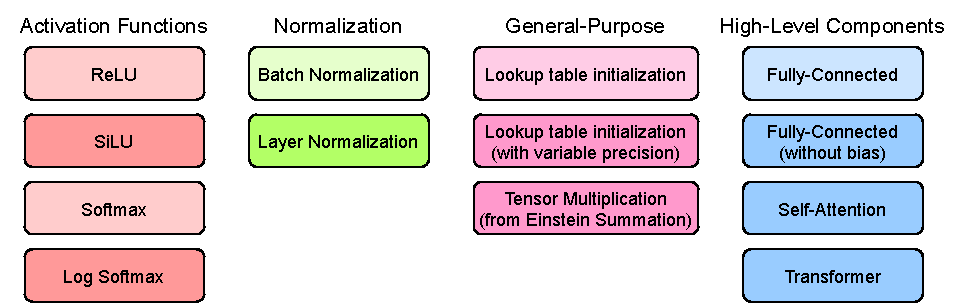
\includegraphics[trim={0cm 0cm 0cm 0cm}, clip, width=0.7\textwidth, center]{quantization/hls4ml_blocks.pdf}
  \caption{Overview of the created implementations (dark-colored) and some existing components with similar functionality (light-colored).}
  \label{fig:hls4ml-contributions}
\end{figure}


\subsection{Activation Functions}
The library offers several common non-linear activation functions, including the basic one - ReLU. An implementation was created for the SiLU, which extends the existing ReLU block by adding multiplication with the sigmoid function that can happen serially or in parallel depending on the specific configuration. In addition, the log softmax activation had implementations developed using both the direct and the optimized method described earlier in this chapter in \cref{log-softmax} to be able to evaluate the success of the optimization process.

\subsection{Normalization Layers}
Layer normalization and batch normalization perform the same operation across different dimensions, which on its own would not require a separate implementation. However, they also differ in terms of statistic collection, as only the batch version collects them during training to use during inference while layer normalization always computes them directly. While this is a suboptimal approach for reconfigurable hardware, a simulation-only version of layer normalization was implemented to allow for analyzing the effect of switching between these two methods to better understand their trade-off.

\subsection{General-Purpose Blocks}\label{hls4ml-general-purpose}
The method used in \hlsml for mapping the precomputed function values to lookup table indexes prioritizes the integer range of a fixed-point number over its fractional part. In other words, it simply uses the \(N\) most significant bits of a value for calculating the table index, where \(N\) is the table word width. Although this approach works in the majority of cases, it limits the ease of exploration as the type used in a lookup table might be affected by another variable's width, hence enforcing an unnecessarily wider integer range and sacrificing decimal precision. A good example is the natural logarithm, which output range can be represented using fewer integer bits than its input domain, which makes it the perfect candidate for using the custom lookup table initialization. Aside from that, the tensor multiplication covered in details in \cref{tensor-multiplication} was implemented in a way to match the style of existing tensor and array modifying components. This makes it very convenient for accelerating more complex designs that rely on Einstein Summation in their PyTorch implementation, and in the future, it could allow \hlsml to automatically translate that concept as it is currently not supported.

\subsection{High-Level Components}
It comes as no surprise that \hlsml offers a customizable and efficient fully-connected layer implementation. However, the way of creating an instance without the bias calculation is to provide an array filled with zeros. This is believed to be a shortcoming of the current version, as having a compile-time parameter regarding the bias can make the synthesis process faster given that the HLS can skip the optimization process for that aspect. With bigger and more complex models, this simple change could lead to noticeable reduction in processing time. What is more, it also yielded a marginally smaller design in the case of this work, suggesting that the HLS hardware translation might not be behaving optimally, but that depends on a number of factors and was not evaluated further.

Although the deeply covered self-attention and transformer layers could be viewed as specific to the topic of this report, it has to be remembered that they are the state-of-the-art when it comes to a plethora of applications. At the same time, they are incomparably more complex than any other aforementioned components, not only needing them for correct functionality, but also requiring considerable amount of development time to properly integrate and carefully optimize. Hence. they are considered the most important \hlsml contributions of this work.